\renewcommand{\SourceFile}{8-vers-la-recursivite/src/8-3.ml}

\section{Les deux points les plus proches}

Le but de ce problème est d'identifier, dans un ensemble de points, quel est le couple de points les plus proches au sens de la distance euclidienne. Ce type d'algorithme voit son utilité dans les transports aériens ou maritimes.
\medskip

L'ensemble de points est vu comme un tableau de 2-tuples de coordonnées $(x,y)$.
\medskip

On dispose de la fonction \texttt{sqrt (x:float) : float} qui renvoie la racine carrée de \texttt{x}.

\Q
Donner un algorithme itératif qui détermine le couple de points les plus proches de l'ensemble.
\medskip

Montrer qu'à chaque itération, votre algorithme répond aux conditions que vous vous êtes fixées (c'est-à-dire vérifie un invariant de boucle).
\medskip

Évaluer le nombre d'additions, de multiplications et d'appels à la fonction \texttt{sqrt}.
\bigskip

L'ensemble de points est stocké dans deux tableaux \texttt{x} où les points sont ordonnés suivant les abscisses croissantes, et \texttt{y} où les points sont ordonnés suivant les ordonnées croissantes.

\Q
Écrire une fonction OCaml \texttt{decoupe (x:point array) (y:point array) (y':point array) (deb:int) (fin:int) : unit} qui place les points du sous-tableau \texttt{x}[\texttt{deb}..\texttt{med}] classés par ordonnée croissante dans le sous-tableau \texttt{y'}[\texttt{deb}..\texttt{med}] et les éléments du sous-tableau \texttt{x}[\texttt{med+1}..\texttt{fin}] classés par ordonnée croissante dans le sous-tableau \texttt{y'}[\texttt{med+1}..\texttt{fin}], où $\texttt{med}=\left\lfloor\frac{\texttt{deb}+\texttt{fin}}{2} \right\rfloor$.
\medskip

Évaluer le nombre de transferts effectués lors de l'exécution de cette fonction.

\Q
Nous supposons que $A$ et $B$ sont les points les plus proches du sous-tableau \texttt{x}[\texttt{deb}..\texttt{med}] et, $C$ et $D$ sont les points les plus proches du sous-tableau \texttt{x}[\texttt{med+1}..\texttt{fin}].
\medskip

Écrire un algorithme linéaire qui détermine les deux points les plus proches de l'ensemble \texttt{x}[\texttt{deb}..\texttt{fin}], connaissant $A$, $B$, $C$, $D$ et \texttt{y}[\texttt{deb}..\texttt{fin}].
\medskip

En déduire une fonction de recherche du couple de points les plus proches (où $A$, $B$, $C$ et $D$ sont déterminés de façon classique).
\medskip

Déterminer la complexité de votre fonction.
\medskip

Que peut-on conclure ?

\Corrige

\Q
Nous proposons un algorithme exhaustif où tous les couples de points sont examinés.

\lstinputlisting[linerange={1-21}]{\SourceFile}

Dans la boucle $i$ : \texttt{p1}, \texttt{p2} est le couple de points les plus proches avec \texttt{p1} pris parmi les $i$ premiers points de \texttt{tab}.\\
Dans la boucle $j$ : \texttt{p1}, \texttt{p2} est le couple de points les plus proches avec \texttt{p1} pris parmi les $i-1$ premiers points de \texttt{tab} avec \texttt{p1=tab.(i)} et \texttt{p2} pris parmi les $j$ premiers points de \texttt{tab}.
\medskip

Le nombre d'additions est $3 \times (n-1)n/2$, de multiplications $(n-1)n$, où $n$ est le nombre de points. Il n'y a pas besoin d'appeler la fonction \texttt{sqrt}.

\Q
Il s'agit simplement de transcrire ce qui est proposé dans l'énoncé :

\lstinputlisting[linerange={23-37}]{\SourceFile}

Le nombre de transferts est de l'ordre du nombre d'éléments de \texttt{x}.

\Q
Suivant les instructions de l'énoncé, le tableau \texttt{x} est découpé en deux parties. Dans chacune d'entre elles, nous avons recherché le couple de points les plus proches.
\medskip

Mais la distance la plus courte peut être donnée par un couple de points à cheval sur les deux parties.
\medskip

Supposons que nous ayons comparé les deux distances et gardé le couple donnant la plus petite distance \texttt{dist}, alors via la fonction \texttt{termine}, nous allons rechercher s'il existe un couple de points pris dans chacune des deux parties, dont la distance est plus petite.
\medskip

Nous reprenons la même terminologie pour les variables.

\lstinputlisting[linerange={39-70}]{\SourceFile}
\newpage

On ne considère que les points contenus dans le rectangle en pointillés, en partant du point le plus bas.

\begin{tikzpicture}[scale=1.1, every node/.style={
    font=\ttfamily,
    draw,
    fill=black,
    circle,
    inner sep=0pt,
    minimum size=5pt}]

    \node at (1,4.3) {};
    \node at (1.4,3) {};
    \node at (2.1,1.2) {};
    \node at (2.15,2.4) {};
    \node at (2.25,4) {};
    \node at (3,3.3) {};
    \node at (3.5,1.6) {};
    \node at (3.95,2.3) {};
    \node at (4,4.25) {};
    \node at (4.75,3.7) {};
    \node at (5.1,1.4) {};
    \node (p1) at (5.9,2.9) {};
    \node (p2) at (6.25,2.4) {};
    \node at (6.8,1.7) {};

    \draw [<->] (p1) -- (p2);
    \node[fill=none, draw=none] (T) at (3.5,5.7) {2d};
    \node[fill=none, draw=none] at (6.35,2.75) {d};
    \node[fill=none, draw=none] at (3.5,-.3) {x.(med)};
    % \node[fill=none, draw=none, rectangle, align=center] at (8,5) {on ne considère que les points\\
    % contenus dans ce rectangle\\
    % en partant du point le plus bas};

    \draw[-latex, thick] (T) -- +(-0.61, 0);
    \draw[-latex, thick] (T) -- +(0.61, 0);

    \draw (3.5,-.1) -- (3.5,5.4);
    \draw[dashed] (2.89,-.08) -- (4.11,-.08) -- (4.11,5.5) -- (2.89,5.5) -- (2.89,-.08);

    \draw[-latex] (0,0) -- (0,5.5);
    \draw[-latex] (0,0) -- (9,0);
\end{tikzpicture}

Si \texttt{d} est la plus petite distance pour chacune des deux moitiés, nous avons au plus 4 points dans un carré de côté \texttt{d}.
\medskip

Ainsi, dans la boucle \texttt{while}, il y a au plus 7 itérations. On représente ici le rectangle examiné dans la boucle \texttt{while} :

\begin{center}
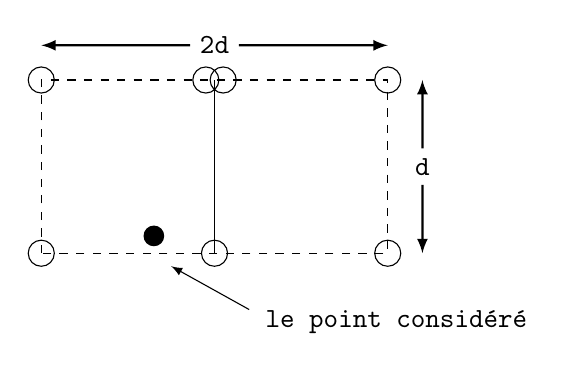
\begin{tikzpicture}[scale=1.1, font=\ttfamily]
    \draw[dashed] (0,0) -- (0,2) -- (4,2) -- (4,0) -- (0,0);
    \draw (2,0) -- (2,2);

    \node[fill=none, draw=none] (T) at (2,2.4) {2d};
    \draw[-latex, thick] (T) -- +(-2, 0);
    \draw[-latex, thick] (T) -- +(2, 0);

    \node[fill=none, draw=none] (R) at (4.4,1) {d};
    \draw[-latex, thick] (R) -- +(0, 1);
    \draw[-latex, thick] (R) -- +(0, -1);

    \node[draw, circle] at (0,0) {};
    \node[draw, circle] at (0,2) {};
    \node[draw, circle] at (4,2) {};
    \node[draw, circle] at (4,0) {};

    \node[draw, circle] at (1.9,2) {};
    \node[draw, circle] at (2.1,2) {};
    \node[draw, circle] at (2,0) {};


    \node[draw, fill, circle, inner sep=2.5pt] at (1.3,.2) {};
    \node at (4.1, -.8) {le point considéré};
    \draw[-latex] (2.4, -.65) -- (1.5, -.15);
\end{tikzpicture}
\end{center}

Nous pouvons ainsi envisager la fonction récursive suivante :

\lstinputlisting[linerange={73-91}]{\SourceFile}

Les fonctions \texttt{decoupe} et \texttt{termine} ont une complexité linéaire (c'est-à-dire en $O(n)$). La complexité de la fonction \texttt{cherche} lorsque \texttt{deb=0} et \texttt{fin=n-1} est donnée par la formule de récurrence suivante : $C(n)=2\cdot C(n/2)+O(n)$.
\medskip

La complexité de \texttt{cherche} est donc en $O(n\log_2n)$.
\bigskip

\Fin
